%%
%% Author: dariochinelli
%% 2021-04-07
%%


\section{Catena unidimensionale di atomi (\textit{dinamica fononica})}
Per questo studio considero una catena unidimensionale, che non è il problema più generale in tre dimensioni da poter risolvere ma generalizza meglio il problema visto nel capitolo precedente sullo studio approssimato di Debye. \\

% ------- ------- ------- ------- ------- ------- ------- ------- ------- ------- -------
Un mezzo solido continuo supporta sia vibrazioni longitudinali sia trasversali, ma Debye ha agito nel modo seguente:
\begin{equation}
\int_0^{\nu_m} N(\nu) d\nu = 3 N_A \Rightarrow \frac{ 4\pi V}{v^3 } \nu_m^3 = 3 N_A
\end{equation}
Ma nel caso più corretto possibile, il solido in questione, soffre di oscillazioni sia trasversali che longitudinali.
Occorre dunque dividere la velocità dell'onda nelle sue componenti.
\begin{equation}
3N_A = \frac{ 3 \pi V}{3 } \nu_m^3 \Bigl(  \frac{ 1}{v_l^3 } + \frac{ 2}{v_t^3 }  \Bigr) \quad\quad \mbox{dove si è usato} \quad
\frac{ 1}{v^3 } = \Bigl(  \frac{ 1}{v_l^3 } + \frac{ 2}{v_t^3 }  \Bigr)
\end{equation}
Dove il 2 sta ad indicare che le onde trasversali hanno due possibili stati di polarizzazione, mentre ce n'è uno solo per le onde longitudinali,
e dunque ciò che abbiamo visto finora vale solo nel caso in cui le onde sono tutte longitudinali, ma ciò non è sempre vero. \\
% ------- ------- ------- ------- ------- ------- ------- ------- ------- ------- -------

Consideriamo quindi una catena unidimensionale di atomi chiusa su se stessa, a \textit{collana}, e detta condizione al contorno di Born–von Karman e cerco di calcolare il numero di modi di vibrazione.
Introduciamo la seguente nomenclatura:
\begin{equation}
\begin{split}
x_n & = \mbox{ posizione $n$-esima particella} \\
R_n & = \mbox{ posizione di equilibrio $n$-esima particella} \\
u_n & = (x_n - R_n) = \mbox{ spostamento dalla posizione di equilibrio } \\
a & = \mbox{ distanza reticolare, distanza fra due posizioni di equilibrio} \\
K & = \mbox{ costante elastica delle molle} \\
\end{split}
\end{equation}
\begin{figure}[h]
\centering
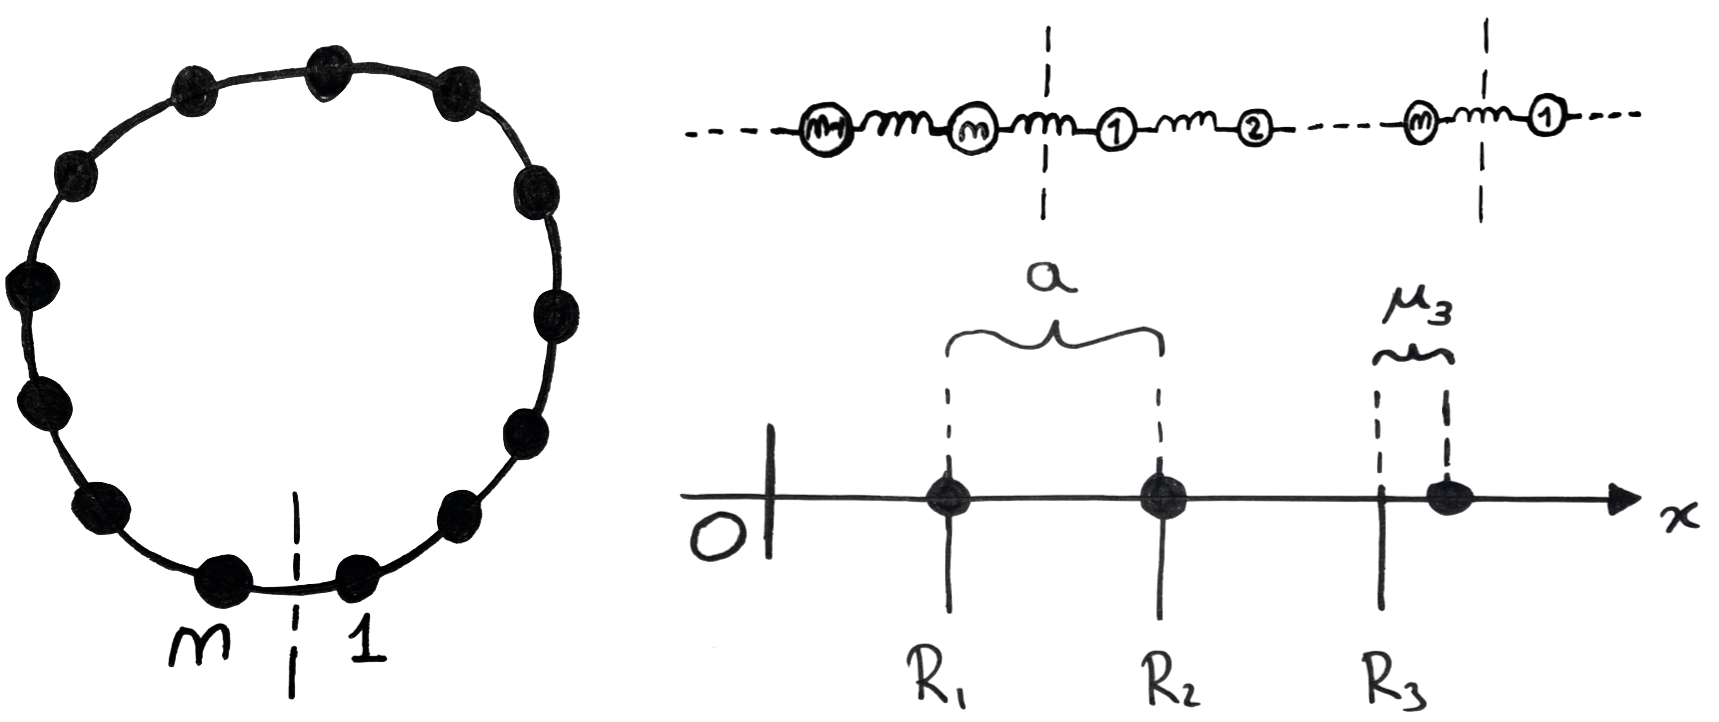
\includegraphics[scale=0.2]{/catena_unidim_atomi}
\caption{Catena unidimensionale di atomi}
\end{figure}
Poiché la catena è chiusa, si impongono condizioni al contorno periodiche.
La forza di interazione tra due particelle è nulla quando la molla è all'equilibrio e cioè quando $x_2-x_1 = a$, quando si trovano ad una distanza $a$, quindi la forza $F_{21}$ che agisce sulla particella $2$ a causa della connessione con $1$
\begin{equation}
\begin{split}
F_{21} & = - K (x_2 - x_1 - a) \\
& = - K (x_2 - R_2 - x_1 + R_1 + R_2 - R_1 - a) \\
& = - K (u_2 - u_1)
\end{split}
\label{forza_F21}
\end{equation}
L'equazione del moto è data da due termini: uno ricavato sopra \ref{forza_F21} ed uno analogo tra la particella $2$ e la particella $3$
\begin{equation}
m \ddot{x_2} = - K (u_2 - u_1) + K (u_3 - u_2)
\end{equation}
la somma è dovuta al fatto che quando la quantità al secondo membro è positiva, l'interazione spinge la particella verso destra sull'asse $x$.
Le derivate seconde $\ddot{x_2} = \ddot{u_2}$ sono equivalenti, per cui è dunque possibile scrivere l'equazione del moto generica per l'$n$-esima particella, 
(sulla quale però si approssima valutando solo le interazioni fra le particelle adiacenti)
\begin{equation}
\begin{split}
m \ddot{u_n} & = - K (u_n - u_{n-1}) + K (u_{n+1} - u_n) \\
& = K \Bigl[  u_{n-1} + u_{n+1} - 2 u_n  \Bigr]
\label{eqmoto_nesimapart}
\end{split}
\end{equation}
La soluzione di questa equazione può essere espressa come onda longitudinale \textit{viaggiante} del tipo
\begin{equation}
u_n = s e^{ i k R_n } e^{ - i \omega t } = s e^{ i (k n a - \omega t) }
\label{solution_un}
\end{equation}
dove
\begin{equation}
\begin{split}
k = \frac{2\pi}{\lambda} \quad \mbox{numero d'onda} \quad\quad&\quad\quad s  = \quad \mbox{ampiezza} \\
\omega = 2 \pi \nu  \quad \mbox{frequenza} \quad\quad\quad\quad&\quad\quad R_n = n a \\
\end{split}
\end{equation}
Sostituendo la soluzione \ref{solution_un} nell'equazione differenziale \ref{eqmoto_nesimapart} dopo aver trovato la derivata 
\begin{equation}
\frac{d^2}{dt^2} u_n = \ddot{u_n} = -\omega^2 s e^{ i ( k n a - \omega t ) }
\end{equation}
ottengo
\begin{equation}
\begin{split}
- \omega^2 m s e^{ i (k n a - \omega t) } & = K \Bigl(  s e^{ - i \omega t }  \Bigr) \Bigl[  e^{ i k (n-1) } + e^{ i k (n+1) } - 2 e^{ i k n } \Bigr] \\
- \omega^2 m s e^{ i k n a } & = K \Bigl[  e^{ - i k a } + e^{ i k a } - 2 \Bigr] e^{ i k n a } \\
\omega^2 m  & = K ( 2 - 2 \cos (k a) )
\end{split}
\end{equation}
utilizzo l'identità trigonometrica: $\sin^2 \frac{ X}{2 } = \frac{ 1}{2 } \Bigl(   1 - \cos(X)  \Bigr)$
\begin{equation}
\omega^2 = \frac{4 K}{m} \sin^2 \frac{k a}{2} 
\quad\Rightarrow\quad 
\omega = 2 \sqrt{\frac{K}{m}} \Bigl| \sin \frac{ka}{2}  \Bigr| \quad\quad\quad \mbox{(da ricordare)}
\label{omega}
\end{equation}
questa formula collega insieme la frequenza $\omega$ ed il numero d'onda $k$.

\paragraph{Studio la funzione in base al valore di $k$} 
Per piccoli numeri d'onda $k$, cioè per grandi lunghezze d'onda $\lambda$, posso approssimare la \ref{omega} con
\begin{equation}
\omega = 2 \sqrt{\frac{K}{m}} \Bigl| \frac{ka}{2}  \Bigr|  \quad\Rightarrow\quad \omega \propto k
\end{equation}
per cui la \textit{velocità di fase}
\begin{equation}
v_{fase} = \frac{\omega}{k}
\end{equation}
è uguale alla \textit{velocità di gruppo}
\begin{equation}
v_{gruppo} = \frac{d \omega}{d k}
\end{equation}
da cui trovo che è indipendente dalla frequenza e vale
\begin{equation}
\frac{\omega}{k} = c = \frac{d \omega}{d k} = \sqrt{\frac{K}{m} a^2}
\end{equation}
allora si dice che \textit{non c'è dispersione}.

Per valori qualsiasi di $k$, uso la \ref{omega} e trovo la funzione $\sin$, periodica su un periodo $2\pi / a$.
La funzione \ref{omega} nell'intervallo $\Bigl[  -\frac{\pi}{a}, +\frac{\pi}{a}  \Bigr]$, detta \textit{"1st Brillouin Zone"}, plottata permette di capire meglio il concetto di dispersione, vedi figura \ref{dispersione} \\
\begin{figure}[h]
\centering
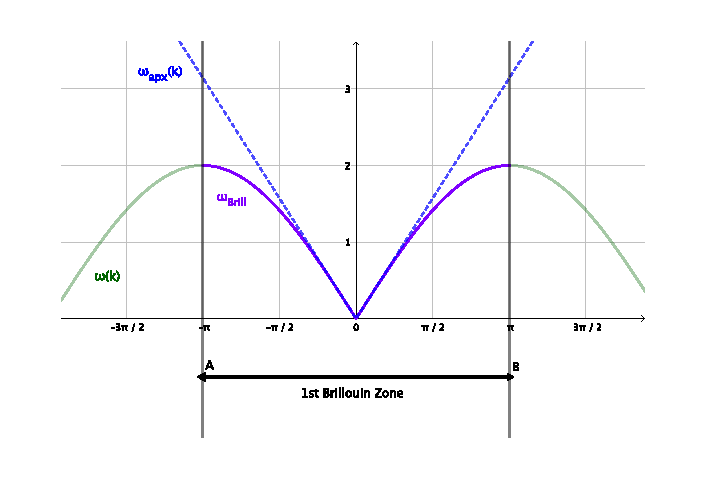
\includegraphics[scale=0.8]{/brillouinzone}
\caption{Curva di dispersione, zona di Brillouin}
\label{dispersione}
\end{figure}
Il distacco tra la funzione lineare e la funzione seno è dovuto al fatto che non ho a che fare con un sistema continuo ma discreto.
Per piccoli $k$ per cui le due curve combaciano, non ho dispersione, mentre per $k$ più grandi le due curve si allontanano e ho dispersione.
Cioè aumentando $k$ non è più vero che la velocità non dipende dalla frequenza e quindi avrò onde a diverse velocità, quindi dispersione.

\paragraph{Condizioni su $k$} avendo considerato una catena di atomi circolare, si dovrà imporre l'uguaglianza tra la funzione relativa al primo atomo e quella relativa all'atomo $N+1$ ovvero
\begin{equation}
\begin{split}
u_1 &= u_{N+1} \\
s \Bigl(  e^{ ika } e^{ -i \omega t }  \Bigr) & =  s \Bigl(  e^{ ik(N+1)a } e^{ -i \omega t }  \Bigr) = s \Bigl(  e^{ ika } e^{ ikNa } e^{ -i \omega t }  \Bigr)
\end{split}
\end{equation}
vera se soddisfa la condizione 
\begin{equation}
e^{ ikNa } = 1
\end{equation}
ovvero
\begin{equation}
k = \frac{2\pi}{N a} l \quad\quad\quad \mbox{quindi} \quad -\frac{N}{2} < l \le \frac{N}{2}
\end{equation}
quindi se $k$ varia di una quantità $\frac{2\pi}{a}$ allora $u_n$ non cambia;
ci sono allora solo $N$ valori di $k$ consistenti con la condizione scritta sopra.


\subsection{Fononi}
In alternativa alla trattazione del capitolo precedente, posso ragionare in termini di particelle per cui ho un modo di frequenza $\omega(k)$ con energia
\begin{equation}
\varepsilon = n h \nu = n \hbar \omega
\end{equation}
e considerare lo stato che contiene $n$ particelle con energia $\hbar \omega$ e numero d'onda $k$
\begin{equation}
\bar \varepsilon = \frac{h \nu}{e^{ \frac{h\nu}{k_B T} } - 1}  
= \frac{\hbar \omega}{e^{ \frac{\hbar\omega}{k_B T} } - 1}  
\end{equation}
tali particelle sono dette \textit{fononi}, descrivibili come i quanti di energia elastica (meccanica), collegata ai moti di vibrazione reticolare.
Sono definite come particelle a \textit{massa nulla} e \textit{spin zero}, sono quindi descrivibili come \textit{bosoni}.
Si può vedere come l'analogo di un fotone: quanto di energia elettromagnetica, ma relativo alle onde elastiche. \\
Utilizzando i \textit{fononi} è possibile trattare alcuni fenomeni di fisica classica e dello stato solido come ad esempio:
\begin{itemize}
\item il calore specifico
\item la resistenza elettrica
\item la trasmissione del calore attraverso un metallo
\item la misura di diffrazione neutronica
\end{itemize}




